\documentclass[titlepage]{article}
\usepackage[norsk]{babel}
\usepackage[utf8]{inputenc}
%\usepackage[latin1]{inputenc}
\usepackage{graphicx}
\usepackage{float}
\usepackage{parskip}
\usepackage{array}
\newcolumntype{L}[1]{>{\raggedright\let\newline\\\arraybackslash\hspace{0pt}}m{#1}}
\newcolumntype{C}[1]{>{\centering\let\newline\\\arraybackslash\hspace{0pt}}m{#1}}
\newcolumntype{R}[1]{>{\raggedleft\let\newline\\\arraybackslash\hspace{0pt}}m{#1}}
\usepackage{longtable}

\author{Gruppe 38}
\title{Prosjektplan}
\date{\today}

\begin{document}

\maketitle

\begin{abstract}
Siden tidenes morgen har samarbeid mellom mennesker skapt verdier. 
\end{abstract}

\tableofcontents


\newpage
\section{Innledning}
Vi skal tilby en forbindelsesorientert nettverksløsning, og dette skal vi gjøre ved hjelp av A1 og A2. A2 eksisterer allerede og er et forbindelsesløst nett. All kontakt mellom klienten og serveren for kalenderapplikasjonen vår skal gå igjennom A1, som deretter tar kontakt med A2 (socketen). Tilkoblingen mot A1 skal være pålitelig og tapsfri, akkurat som TCP. Vi skal endre på ConnectionImpl-klassen som implementerer Connection-klassen. Det er 4 sentrale metoder vi skal impelentere. Disse er accept(), connect(address, port), close(), send() og receive(). Om vi skulle ønske, og ha behov, kan vi også implementere isValid(packet). A1 skal kommunisere med A2 gjennom metodene send, receive og cancel\_receive som ligger i A2.

For å kunne opprette en pålitelig tilkopling igjennom A2, må vi selv opprette koplinger for data som skal sendes. Når dette er gjort kan vi sikre tapsfri overføring. I sekvensdiagrammene vi har laget, viser vi hvordan serveren og klienten kan abstrahere bort mange funksjoner som alltid må kjøres, og dermed bare konsentrere seg om det essensielle. Vi viser spesifikt tilfellene Connect, Send og Close.

Når vi oppretter en connection skal det utføres en three-way-handshake. Først sender vi en SYN fra klienten til servern, i respons får vi en SYN-ACK tilbake, og tilslutt sender klienten en ACK til servern og det har blitt dannet en tilkobling.

Hver gang en pakke blir sendt så sender man med et sekvensnummer, deretter får man tilbake en ACK og hva mottakeren forventer at neste sekvensnummer skal være, dermed vet man at pakken kom fram. 
Når en tilkobling skal bli lukket vil det utføres en three-way-handshake her også. Dette foregår ved at klienten sender en FIN mot servern, som vil svare med ACK (servern har fått pakken) og en FIN selv. Klienten får dette tilbake og svarer da med en ACK selv, og tilkoblingen blir avsluttet.
For å kunne lage en god kommunikasjon, er det fint å vite hva som finnes i A2. Dette kan aksesseres ved å bruke Admin-klassen. Vi kan her skrive ut logger fra A2 og gjøre innstillinger. Med disse verktøyene kan vi lage en pålitelig og god tilkopling.

\newpage
\section{Ansvarsfordeling}
\subsection{Inndeling}
\textbf{Scrummaster}: Juul Arthur\\
\emph{Scrumvikar}: Per Øyvind\\
SU: Julian\\
MMI: Heidi, Julian\\
KTN: Christoffer, Tino\\
DB: Per Øyvind, Juul Arthur

\subsection{Begrunnelse}
Vi har fordelt personene i gruppen til ulike fagområder. Personen(e) som er satt til de ulike fagområdene har ansvar for at oppgavene blir gjort, og vil også være de som fordyper seg mest i emnet. Alle gruppemedlemmene skal være aktive i hvert fagområde og bidra på alle øvingene. Dersom noen blir ferdig med sin oppgave tidligere, så skal de hjelpe til med pågående oppgaver.

\newpage
\section{GANTT-diagram}
\begin{figure}[H]
\label{fig:gantt}
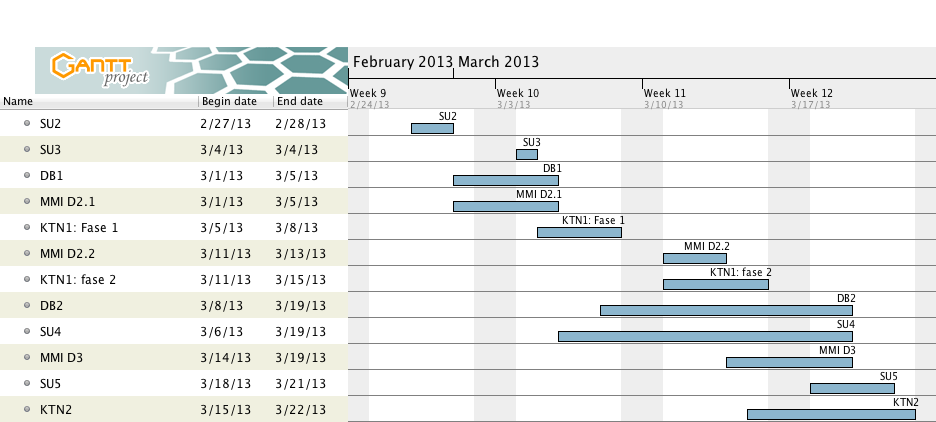
\includegraphics[width=400px]{Gantt-diagram.png}
\caption{GANTT-diagram for arbeidet}
\end{figure}

\newpage
\section{Arbeidspakker}
\begin{center}
\label{tab:arbeidspakker}
\begin{longtable}{| l | l |}
\hline
Pakke & Timer\\
\hline
SU2: Funksjonelle krav & 12 \\
\hline
SU2: Ikke-funksjonelle krav & 12 \\
\hline
DB1: ER-modell & 16 \\
\hline
SU3: Scenario 1 & 4 \\
\hline
SU3: Scenario 2 & 4 \\
\hline
SU3: Scenario 3 & 4 \\
\hline
SU3: Klassediagram & 8 \\
\hline
MMI D2.1: Idémyldring & 3 \\
\hline
MMI D2.1: Papirmodell & 4 \\
\hline
KTN fase 1: Sekvensdiagram & 2 \\
\hline
KTN fase 1: Tilstandsdiagram & 4 \\
\hline
KTN fase 1: Tekstlig beskrivelse & 6 \\
\hline
KTN fase 1: Feilhåndtering & 6 \\
\hline
KTN fase 1: Testplan & 12 \\
\hline
MMI D2.2 & 16 \\
\hline
KTN fase 2: Feilretting & 16 \\
\hline
DB2: Design & 8 \\
\hline
DB2: SQL som gjør noe & 8 \\
\hline
DB2: SQL & 16 \\
\hline
DB2: Testing/fiksing & 12 \\
\hline
SU4: Logg på/av & 16\\
\hline
SU4: Avtale & 16\\
\hline
SU4: Møteinnkalling & 16\\
\hline
SU4: Avlyse/melde avbud møte & 10\\
\hline
SU4: Møterom & 6\\
\hline
SU4: Visning & 16\\
\hline
SU4: Alarm & 6\\
\hline
MMI D3: Skjermbilde & 16\\ %OBS OBS! Stemmer dette?
\hline
MMI D3: Konseptuellmodell & 16\\
\hline
MMI D3: skjermdesign & 16\\
\hline
MMI D3: Konstuksjonsbeskrivelse & 16\\
\hline
SU5: Sluttrapport tidsestimering & 4\\
\hline
SU5: Systemtestrapport & 16\\
\hline
SU5: Prosjekterfaringer & 6\\
\hline
Total: & 349\\
\hline
\caption{Oversikt over arbeidspakkene våre}
\end{longtable}
\end{center}

\newpage
\section{Sprint}
\subsection{Sprint 1}

\newpage
\section{Risikoanalyse}
\subsection{Risikoscenarioer}
\begin{center}
\label{tab:risikoscnarioer}
\begin{longtable}{| l | L{4cm} | L{4cm} | L{4cm} |}
\hline
ID & Situasjon & Forebyggende tiltak & Løsningsplan \\
\hline
1 & En eller flere personer er ikke interessert i å bidra, kommer ikke til planlagte møter, vanskelig å få kontakt med. & Være inkluderende på møter. Prøve å variere på arbeidsoppgaver så ingen går lei. Forståelse for at kompetansen i gruppen kan variere veldig. & SCRUM-master tar direkte kontakt med personen,bytte oppgaver hvis personen er misfornøyd, evt ta kontakt med und.ass/faglærer og avtale møte som alle i gruppen må delta på.\\
\hline
2 & Tidsestemering slår feil. En eller flere oppgaver er mye mer tidskrevende enn antatt. & Ha møte hver morgen der vi forteller om hva vi har gjort og eventuelt om noe var mer tidkrevende enn først antatt. Møter med und.ass hvor vi får tips om hvilke oppgaver vi burde sette av mest tid til. & Sette av mer tid til oppgaven. Kompensere ved å ha flere arbeidstimer (vurdere overtid), eventuelt omallokere ressursene våres. Droppe noen ikke-essensielle krav for oppgaven. Diskutere på møte hvorfor tidsestemeringen gikk galt, og lære av dette. \\
\hline
3 & To eller flere gruppemedlemmer misliker hverandre sterkt, og nekter å samarbeide. Skader produktiviteten og gruppemoralen. & God dialog innad i gruppen. Personer som ikke samarbeider bra blir satt til forskjellige arbeidsoppgaver. & Først prøve en gruppesamtale, hvor SCRUM-master prøver å løse konfliktene.
Samtale med und.ass, foreslå bytting av grupper hvis nødvendig. \\
\hline
4 & En eller flere personer tar på seg en for stor oppgave. Blir veldig skeiv arbeidsfordeling, noen gjør mye mer enn andre. & Snakke om hva alle har gjort siden sist på hvert møte. Inkludere alle i planleggingen, og passe på at ingen tar oppgaver de ikke har kompetanse til å håndtere. Sørge for at oppgavene er jevnt fordelt utover alle gruppemedlemmer. & Omrokkere på arbeidsoppgaver og sørge for bedre dialog. Ta det opp på møtet. \\
\hline
5 & Alle i gruppen har \underline{ikke} aktive arbeidsoppgaver til en hver tid. & Kartlegge kompetansen veldig tidlig, og alltid ha dette i bakhodet ved delegering av oppgaver. Fortelle om arbeidsoppgavene våres for dagen på daglige møter. Være aktive på IRC. Sørge for at vi har en gruppefølelse og at vi har lyst til å lykkes sammen. & Sette personer som ikke har arbeidsoppgaver over til nye arbeidsoppgaver, eventuelt hjelpe andre som fortsatt har flere oppgaver igjen. \\
\hline
6 & Kompetansen til de ulike medlemmene blir ikke brukt på en effektiv måte. & Da har vi ikke gjort en god nok jobb i forhold til punkt 5 og må ta det opp på morgenmøtet for å løse problemet. & . \\
\hline
7 & Uforventet fravær fra ett/ flere gruppemedlemmer. & Vi må være aktive i å informere om noe forekommer. & Omallokere arbeidsoppgaver og prioritere arbeidsoppgaver som er viktigere. Sette av mer tid til oppgavene. \\
\hline
\caption{Tabell med oversikt over risikoanalysen vi har foretatt}
\end{longtable}
\end{center}

\subsection{Scenariovurdering}
\begin{table}[H]
\centering
\label{tab:scenariovurdering}
\begin{tabular}{| l | l | l |}
\hline
ID & Sannsynlighet & Alvorlighetsgrad \\
\hline
1 & Liten & Alvorlig \\
\hline
2 & Svært stor & Liten \\
\hline
3 & Moderat & Alvorlig \\
\hline
4 & Stor & Moderat \\
\hline
5 & Stor & Liten \\
\hline
6 & Moderat & Moderat \\
\hline
7 & Stor & Moderat \\
\hline
\end{tabular}
\caption{Tabell med oversikt over scenariovurdering}
\end{table}

\newpage
\listoftables

\newpage
\listoffigures

\newpage
\begin{thebibliography}{9}

\bibitem{fpkomp}
	Kompendium til fellesprosjektet,
	\emph{it's learning-gruppa til faget}
\end{thebibliography}

\end{document}
